% Generated by thesis/ch7/exp1/make_figures.py -- do not edit by hand.
\begin{figure}[tbp]
  \centering
  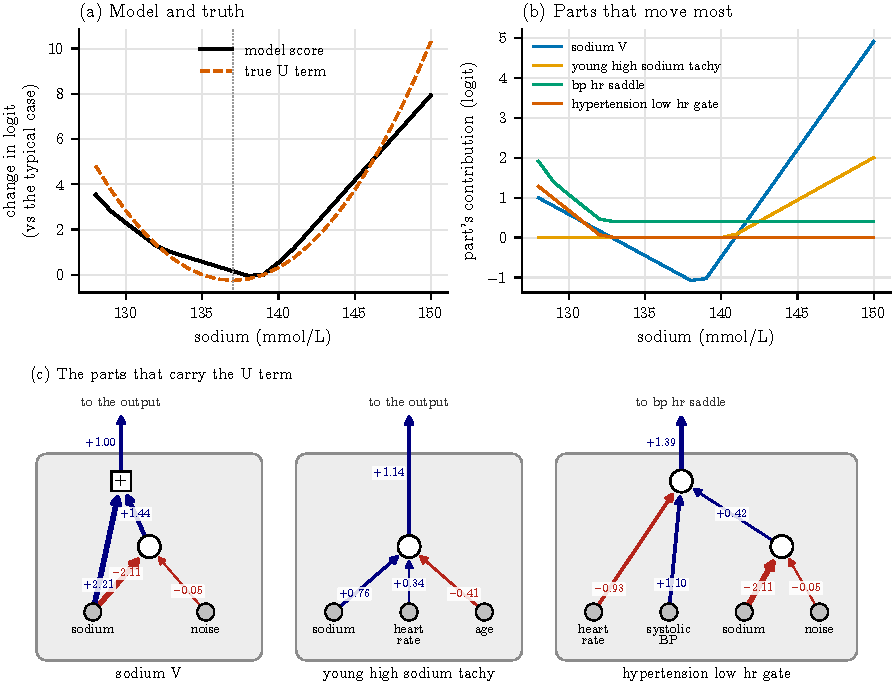
\includegraphics[width=\textwidth,height=0.8\textheight,keepaspectratio]{figures/ch7/synthetic-shape-c-sodium.pdf}
  \caption{Synthetic U + saddle network (seed 4): the U-shaped sodium term. (a) Black: the model's score as sodium varies, every other input at the typical case, relative to the typical sodium; dashed: the true U term $((z_n - (-0.5))^2 - 1)$, lowest at 137 mmol/L; dotted: 137 mmol/L. (b) The explanation parts whose contribution moves most with sodium. (c) The network's parts that carry the U term: grey box: one part of the explanation (its name below); small grey circles: the inputs it reads; white circles: hidden units (ReLU); square $+$: the part's sum (no activation). Edges: blue, a positive weight; red, a negative weight; thicker, a larger weight; the number on an edge is its weight. Arrows leaving a box: the part's connections to the rest of the network, labelled with what they feed.}
  \label{fig:ch7-synthetic-shape-c-sodium}
\end{figure}
